\chapter{Aurelia: Scalable CXL fabric}
\label{aurelia:chap}

%\section{Introduction}
%\stingw{the idea is to use CXL fabric as the next-gen rack-scale fabric for disaggregation/composable systems.}
%\stingw{why do we need CXL at the first place? disaggregation and composable system}
% \TODO{Steve: I'm not sure how to parse this.  If "datacenters" should be possesive, it's not a sentence.  If "datacenters" is plural, it's awkward to call them "the" datacenters.}
%
With the trend toward disaggregation and composable infrastructure, different resources in datacenters are taken from a logical pool to satisfy the demand from applications.
%
Existing efforts of disaggregation relies on RDMA over Ethernet, a fabric not designed with disaggregation in mind~\cite{legoos:osdi:2018, far-memory:eurosys:2020, leap:atc:2020,aifm:osdi:2020,carbink:osdi:2022,hydra:fast:2022,canvas:nsdi:2023}.
%
However, retrofitting existing hardware prevents applications from achieving their optimal performance under disaggregation. 
%and sometimes demonstrates inferior performance. 
%than its counterpart 
%
%\TODO{Steve: what counterpart?}
%
%with server-based setups.

Recent works focus on co-designing hardware with software to realize disaggregation~\cite{kona:asplos:2021, intel-cxl:ieee-micro:2023, tpp:asplos:2023, pond:asplos:2023}.
%
These works focus on externalizing hardware interconnects to create a fabric that connects many devices in a disaggregated setting
%
Fabrics directly connect all the devices allowing access to remote devices in a manner similar to accessing local devices on a server's PCIe slots.  
%
PCIe is an example of this type of fabric, but it currently only connects local devices within a server.
%
% For inter-server communication, PCIe is mainly used to pass data to NIC that further passes the data over Ethernet. 
%
%\stingw{PCIe can go across servers with non-transparent bridge but it's hardly used.}
%
An ideal fabric for disaggregation offers direct connections between devices while providing low latency and high bandwidth at a specific scale, e.g. a single rack or a few neighboring racks.
%rich semantics beyond PCIe's I/O semantics 

ompute Express Link (CXL) has emerged as a viable candidate, supported by a converged industry standard following its absorption of OpenCAPI and Gen-Z.
%
CXL is built on top of PCIe with the addition of memory accessing semantics (CXL.mem), caching semantics (CXL.cache), and peer-to-peer memory access between devices (Unordered I/O in CXL.io). 
%
% \stingw{CXL-capable devices use load/store to access everything without any software layering}
%
More importantly, CXL can be a fabric through its support of multi-level switching.

Experimental CXL fabric demonstrates on-par performance with lower cost in the case of machine learning model training on tens of GPUs~\cite{fabric-saving}.
%
CXL fabric offers bandwidth as high as 63 GB/s with PCIe 5.0 now and 121 GB/s PCIe 6.0 on the horizon within the next two years~\cite{pcie-6-7}.
% https://www.xda-developers.com/pcie-6-to-launch-in-2024-pcie-7-in-2027/
%
%CXL fabric is able to offer performance benefit from the fabric adoption atop of proper right-sizing of hardware due to disaggregation.
%
CXL fabric offers low latency by operating on a device-attached interface that uses direct load/store instructions.
%to avoid additional interface transition. 
%(CXL $\rightarrow$ CXL). 
%
It avoids the network software stack overhead and the PCIe transition between device and NIC on the sending (Device $\rightarrow$ PCIe $\rightarrow$ NIC) and receiving (NIC $\rightarrow$ PCIe $\rightarrow$ Device) path.
%
The network stack and PCIe transition create latency overhead and throughput bottleneck.
%
First, the network stack using kernel bypassing still incurs latency overhead in the range of microseconds~\cite{shinjuku:nsdi:2019, shenango:nsdi:2019, eRPC:nsdi:2019,snap:sosp:2019}.
%
Second, the PCIe latency overhead of 1500 B packets reaching the wire can be as high as 77\%~\cite{pcie-bench:sigcomm:2018}.
%
Third, the PCIe link to NIC is a potential throughput bottleneck when multiple devices share the NIC.
%
Dedicating a NIC for each device circumvents the throughput bottleneck but at the cost of requiring more NICs and switches. %with the increased cost on more NICs and switches.

%\vspace{-1ex}
\section{Motivation and Background}
\label{aurelia:sec:motivation}

% \TODO{Steve: You genenarly should not have a subsub section  starting immediately after a subsection.  You need some kind of introductory paragraph.    The same applies for subsections with sections and other levels of the document hirerarchy.}

% \subsection{What is CXL?}
Compute Express Link (CXL) has emerged as an enhancement of PCIe, providing cache coherency (CXL.cache), host-managed or fabric-attached memory (CXL.mem), and peer-to-peer memory access between I/O devices (CXL.io).
%
CXL.mem provides host-managed memory that CPU and accelerators are able to read/write into each other's memory directly. 
%
This avoids redundant DMA operations for moving data back and forth~\cite{fulcrum:hpca:2020, beacon:micro:2022, intel-cxl:ieee-micro:2023}.
%
CXL.mem enables fabric-attached memory providing a shared memory pool for applications with different demands~\cite{cxl-ssd:hotstorage:2022, directcxl:atc:2022, pond:asplos:2023}.
%
CXL.cache supports a fully coherent cache on the devices.
%
These devices, however, do not open their local, private memory to CXL-capable hosts. 
%
CXL.io uses unordered I/O for peer-to-peer memory accesses between non-coherent devices over its fabric.
%
%CXL.io supports non-coherent data movement with I/O devices like PCIe does.

\noindent \textbf{Fabric Routing.}
%
CXL routes packets with a per-device ID called Port ID on the fabric. 
%
The Port ID-based routing (PBR) addresses each device with a 12-bit ID. 
%
A packet using PBR contains a specific source port ID and destination port ID before it leaves an edge CXL switch that directly connects with devices.
%
Each CXL fabric has a single fabric manager responsible for initializing, binding/unbinding devices to ports, and handling event notifications, such as device removal or failure, from the switch.
%
This fabric manager functions similarly to a centralized network controller, as it controls per-port forwarding and is aware of all route changes.

\noindent \textbf{Flow control.}
CXL inherits point-to-point flow control from PCIe, which was designed for communication between the device and CPU rather than for a fabric.
%
The flow control operates between two directly connected endpoints.
%
They exchange credit tokens to evaluate the available buffer space on each side.

\noindent \textbf{QoS Telemetry:.}
CXL fabric offers a rate throttling mechanism for hosts called QoS Telemetry.
%
It is used for devices with local memory, including memory expansion devices and accelerators with device memory, such as GPUs, FPGAs, and ASICs.
%
QoS telemetry enables memory devices to indicate their current internal load with 2 bits in CXL.mem response packets.
%
Senders use the reported internal load to monitor and throttle their request rate to avoid device overload and potential fabric congestion.
%
The rate throttling specifically targets devices, mainly memory devices, that are associated with a host in the current design.
%
In addition, QoS telemetry includes a mechanism called Egress Port Backpressure (EP Backpressure).
%
It monitors the flow control backpressure situation on each CXL switch egress port.
%
If the port cannot transmit packets for a period of time due to a lack of credits, it marks the EP Backpressure value with 2 bits in the device load field of the outgoing request.
%
The overall load of a device is determined by the maximum of the device's internal load and EP Backpressure.

\subsection{What is Different with CXL Fabric?}
% \stingw{1. latency (synchronous request) and scalability (cache coherence plague + routing + transport)}
CXL fabric exposes memory traffic that used to be internal to a server to all endpoints connected to the fabric.
%
The memory traffic, such as cache coherence, memory access, and I/O-style accesses, runs between processor and device endpoints on the CXL fabric.
%
This contrasts with standard datacenter traffic, which runs with encapsulated packets from per-server NICs outside the internal memory fabric of a server.
%
Processors and accelerators access remote devices using load/store instructions through the CXL fabric.
%
They synchronously request data from remote devices, such as memory expansion modules, accelerators, and storage devices.
%
However, these synchronous data requests cannot tolerate significant latency, as it will stall the execution of the requesting hardware while awaiting the requested data.
%
This poses stringent latency requirements for the fabric and necessitates proper system-level support.
%
Additionally, the CXL fabric supports up to 4096 endpoints.
%
Given the scale of thousands of endpoints and the mixture of memory traffic, this introduces a challenge to the scalability of the underlying protocol design.
%
A centralized scheduler is a possible solution for tens or even hundreds of endpoints on racks.
%
However, the scheduler is very likely to become a performance bottleneck because it needs to sustain and determine the order of every load/store instruction.
%
The scheduler can also become a single point of failure for all memory traffic.
%
A centralized design for the scheduler limits the scalability of CXL, especially when using a longer-distance physical layer compared to PCIe.
%
% \TODO{Why not just make it a scheduler instead of distributed protocols?}
% \stingw{We try tot argue this qualitatively.}
%
To understand the practical challenges, use cases of the CXL fabric from the CXL specification and the literature are discussed next~\cite{cxl-3-0-spec, directcxl:atc:2022, pond:asplos:2023}.
%

\subsection{Use Cases of CXL Fabric}
\label{aurelia:subsec:use-cases}
The use cases of CXL fabrics demand large memory capacity, high bandwidth, and low latency.
%
Emerging and existing workloads in datacenters, such as machine learning models, 
large-scale key-value stores, and high-performance computing (HPC) applications, can benefit from CXL fabrics.   

% Moreover, CXL fabric provides an alternative to Nvidia's proprietary stack (NVLink + NVSwitch + Infiniband RDMA).
% %
% CXL fabric will enable future accelerators to connect and cooperate on applications on a shared, open-standard communication substrate
% instead of using only GPUs.
%
% \TODO{cite NERSC's Arxiv report to argue for the need of disagg with concrete numbers.}
%
%HPC uses a topology like model training but featuring different 
% Host CPU cores are connected with accelerators and accessing fabric-attached memory for additional memory capacity and bandwidth~\cite{memory-trend:snl:2020, hpc-disagg-mem:arxiv:2023} (Shown in Figure~\ref{fig:ml-acc-cxl}).
% Previous works proposed to leave these out of accelerators onto main memory but with potential slowdown caused by explicit memory copying from memory to accelerators~\cite{zero-infinity:sc:2021, zero-offload:atc:2021, deepspeed-inference:sc:2022}.

First, current machine learning models require a large amount of memory on an accelerator, such as a GPU or TPU, which is beyond the capacity of individual accelerators.
%
To make matters worse, the size of state-of-the-art machine learning models ranges from tens of GB to tens of TB~\cite{zero:arxiv:2020, zero-infinity:sc:2021, zionex:isca:2022} and continues to grow every few months.
%
Training and inference of machine learning models now require multiple accelerators to jointly fit the model and intermediate variables into their memory.
%
The CXL fabric could expand accessible memory for accelerators by providing fabric-attached memory.
%
Fabric-attached memory increases the memory capacity and bandwidth to all available memory on the fabric~\cite{cxl-3-0-spec, samsung-memory-expander:hcs:2022, memory-scalability:microchip}.
%
%A topology of this model training use case is shown in Figure~\ref{fig
%
A host is connected with an accelerator with CXL, and they share a coherence domain (Shown in Figure~\ref{fig:ml-acc-cxl}).   
%
Accelerators access the fabric-attached memory and each other's memory in a producer-consumer fashion of I/O coherency.
%

Second, datacenters run cloud services with key-value stores.
%
% \TODO{Steve: This is a pretty sweeping statement and is not true in general.  You can just say "most" or, even better, "many".}
Many high-performance key-value stores use RDMA inside data centers to speed up communication and operations~\cite{farm:nsdi:2014, herd:sigcomm:2014, eRPC:nsdi:2019, xstore:osdi:2020}.
%
These operations are sensitive to latency and are on the performance-critical path of applications.
%
DirectCXL demonstrated that CXL has 8.3x lower latency than RDMA for 64B reads and incurs less overhead when replacing RDMA~\cite{directcxl:atc:2022}.
%
DirectCXL provides a lower bound on CXL latency because its fabric uses a single switch and is not subject to stress or congestion.
%
Hosts do not maintain cache coherence between themselves. 
%
Instead, the fabric-attached memory module maintains coherence between itself and the host address space it has mapped. (Shown in Figure.~\ref{fig:kvs-cxl}).

Third, HPC workloads demonstrate high utilization (greater than 90\%) of memory bandwidth as well as capacity for representative applications~\cite{doe-miniapps, crossroad-benchmarks, exascale-apps}.
%
However, each application reaches its peak memory usage for different durations.
%
The cluster must be provisioned to accommodate peak bandwidth and capacity to avoid significant slowdowns~\cite{hpc-memory-requirement:upc:2019, memory-trend:snl:2020, hpc-disagg-mem:arxiv:2023}.

Machine learning and HPC workloads both involve collective communication, while key-value stores involve bursty, non-structural communication.
%
Collective communication is structural and can be optimized with data prefetching to minimize stalls on pending memory accesses.
%
This relaxes their requirements on latency and reduces burstiness.
%
Training and inference of machine learning models use all-reduce operations to update model weights across each accelerator after each iteration. The size of state-of-the-art models ranges from tens of GB to tens of TB~\cite{zero:arxiv:2020, zero-infinity:sc:2021, zionex:isca:2022}.
%
HPC workloads, compared to machine learning, have a more diverse communication pattern, such as sweeping or nearest-neighbors~\cite{mpi-usage:sc:2019, ember-comm, exascale-apps, doe-miniapps}.
%
Key-value stores and databases, however, serve bursty requests and are sensitive to latency~\cite{scale-memcache:nsdi:2013, rocksdb-modeling:fast:2020}.

\begin{figure}[ht!]
%%%%
    \begin{subfigure}[ht]{0.8\columnwidth}
    \centering{
    \includegraphics[width=\columnwidth]{./figure/aurelia/ml-acc-cxl-fabric.pdf}
    \caption{Machine learning and HPC. Hosts and their accelerators share a coherent domain.}
    \label{fig:ml-acc-cxl}
    }
    \end{subfigure}

    \begin{subfigure}[ht]{0.8\columnwidth}
    \centering{
    \includegraphics[width=\columnwidth]{./figure/aurelia/kvs-cxl-fabric.pdf}
    \caption{Key-value store for cloud services.}
    \label{fig:kvs-cxl}  
    }
    \end{subfigure}
\caption{CXL fabric abstractive topology. Each solid line connecting to CXL fabric is 16 lanes of PCIe 5 or PCIe 6 with a total bandwidth of 128 GB/s or 256 GB/s.}
\label{fig:cxl-topo}
\end{figure}

% \begin{table}[ht!]
% \begin{tabular}{|l|l|l|l|}
% \hline
%             & Bandwidth & Latency & Burstiness         \\ \hline
% Machine Learning Models & +         & $\triangle$    & -           \\ \hline
% High Performance Computing        & +         & $\triangle$    & $\triangle$ \\ \hline
% Key-value Store    & -         & +              & +           \\ \hline
% \end{tabular}
% \caption{Traffic patterns for different workloads.}
% \label{tab:cxl-workload}
% \end{table}

\section{Challenges}
% \begin{comment}
% list out the challenges related to scalability and latency
% latency     -> congestion control, long stall
% scalability -> routing, coherence traffic monitoring + restriction if possible     
% \end{comment}
%
The current design of the CXL fabric~\cite{cxl-3-0-spec} poses challenges regarding scalability and latency.
%
First, its addressing and routing design limits the possibility for flexible and dynamic routing.
%
Second, the lack of an end-to-end transport layer in the fabric makes it prone to congestion and latency spikes.
%
More importantly, with the use of load/store instructions, processors and accelerators that synchronously request data are highly sensitive to latency, as it determines how long they need to stall their execution.
%
The challenges related to addressing, routing, and transport layers are discussed in the following subsections.

\subsection{Addressing and Routing Challenges}
\label{aurelia:sec:motivation:routing}

%\noindent \textbf{Routing.}
CXL routes packets with a per-device ID called Port ID on the fabric. 
%
The Port ID-based routing (PBR) assigns each device a 12-bit ID.
%
A packet with PBR contains a specific source port ID and destination port ID before it leaves an edge CXL switch that connects directly with devices.
%
Each CXL fabric has a single fabric manager to initialize, bind/unbind devices to ports, and handle event notifications, such as the removal or failure of devices, from the switch.   
%
The fabric manager is similar to a centralized software-defined network controller as it controls the per-port forwarding and is aware of all the route changes. 
%
However, the CXL fabric has (1) a limiting addressing scheme that is hard to support multi-path and adaptive routing, and 
(2) single-path and inactive routing regardless of the traffic condition.

%However, the current CXL routing falls short to achieve its own expectation because of the following reasons.
\noindent \textbf{Challenge: Limited addressing support for multi-path and adaptive routing.}
%
% \stingw{ Yes multi-level routing is feasible with CXL 3.0.
% But SPID and DPID are only used to describe devices.
% The fabric routing is SDN-style, so all routing reconfiguration (with packet sparying or load aware) needs to go through Fabric Manager. This make FM a performance bottleneck.
% }
%
The current PBR routing scheme assigns an ID to devices only. 
%
PBR routes packets to the destination device through multi-level switches with routing installed by the fabric manager. 
%
Any routing reconfiguration needs to go through the fabric manager, making load-aware, adaptive routing inefficient and infeasible on a large scale.
%
%PBR with routes controlled by the fabric manager 
The centralized routing of PBR prevents the usage of classic multi-pathing techniques like packet spraying or ECMP because all the routes are pre-determined by the fabric manager.
%
Figure.~\ref{fig:cxl-fabric-overview} shows an example of multi-level CXL fabric.     
%
%if the fabric does not have inter-switch links with a single-level switching.
%
% PBR prevents CXL fabric to realize the multi-level switching that enables a larger topology with switches connected.
%
%PBR cannot route packets through this because it does not address the switches on the fabric.  

\noindent \textbf{Challenge: inflexible routing over diverse topologies.}
CXL fabric supports flexible topology and thus opens the possibility of having a wide range of topologies such as a fully connected graph, fat-tree~\cite{fat-tree:sigcomm:2008}, Dragonfly~\cite{dragonfly:isca:2008}, or reconfigurable topology~\cite{string-figure:hpca:2019}. 
%
These topologies provide multiple paths for a source and a destination, but CXL fabric cannot route packets over multiple possible paths given its current design.

\subsection{Transport-level Challenges}
\label{aurelia:sec:motivation:transport}
% The transport of CXL includes PCIe for point-to-point flow control and QoS Telemetry implementing ad hoc rate-throttling for CXL.mem traffic. These two mechanisms are not able to ensure a predictable fabric latency with minimal congestion.  

CXL inherits point-to-point flow control from PCIe, which was designed for the communication between the device and CPU rather than for a fabric. 
%
The flow control operates between two directly connected endpoints. 
%
They exchange credit tokens to evaluate the available buffer space on each side. 
%

\begin{figure}[t!]  
    \centering
    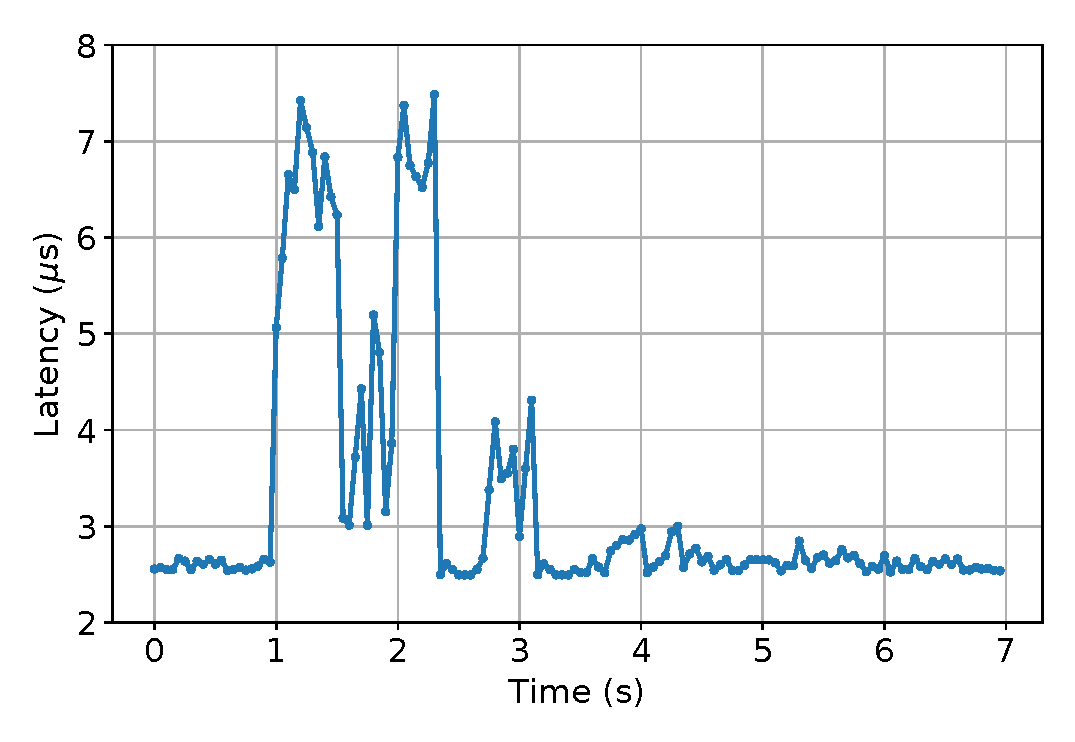
\includegraphics[width=0.8\columnwidth]{figure/aurelia/pcie-congestion.eps}  
    \caption{    
    Congestion on a shared PCIe switch port causes latency spikes of RDMA writes going through the port.      
    %RDMA latency spikes almost 3 $\times$ by PCIe congestion.
    %\TODO{Steve: I don't know what this means.} \TODO{we need better descriptions for this}
    }
    \label{fig:pcie-congestion}        
\end{figure}

\noindent \textbf{Challenges: Flow control cannot prevent congestion.}
The point-to-point, credit-based flow control is focused on preventing buffer overruns only. 
%
It cannot handle pairs of endpoints sharing a port on the switch because no information is exchanged between them.

\noindent \textbf{PCIe congestion experiment.}
We design an experiment of multiple flows sharing a port on a switch, and creating congestion.
%
Given the lack of commercially available hardware for CXL 3.0, we use PCIe, which shares the same flow control mechanism, for our experiment. 
%
Interestingly, PCIe congestion has been identified and demonstrated under various setups~\cite{sbfc:ieee-micro:2005, pcie-congestion-model:sc:2016, invisible-probe:oaklnad:2021}. 

We create artificial PCIe congestion on a PCIe switch port shared by two devices. 
%
The machine uses a SuperMicro X11SPA-TF motherboard with a Broadcom PEX8747 PCIe switch. 
%
The PCIe switch has one upstream port to the CPU and two downstream ports connecting to the devices: An Nvidia 2080 Ti GPU and a ConnectX-5 RDMA NIC.
%
\begin{figure}[ht!]  
    \centering
    %includegraphics[width=1\columnwidth, cframe=red!5!red 0.5mm]{figures/pcie-exp.eps}  
    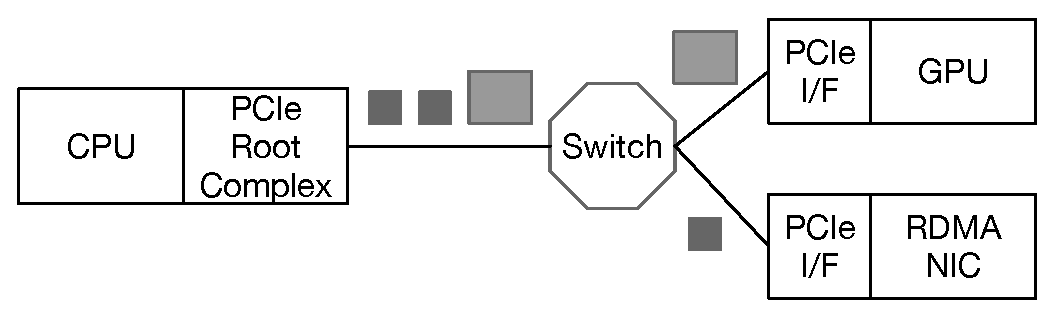
\includegraphics[width=0.8\columnwidth]{figure/aurelia/pcie-exp.eps}  
    %\vspace{-2ex}
    \caption{Experimental setup for PCIe congestion.}
    \label{fig:pcie-experiment}        
\end{figure}
%
The PCIe switch connects with the host processor on one side and provides two ports connecting to GPU and RDMA NIC.
%
The experimental setup is shown in Figure~\ref{fig:pcie-experiment}.
%
During the experiment, the NIC periodically sends RDMA write requests to another machine every 100 microseconds. 
%
Each write request is sent from the CPU and travels through the PCIe switch to the NIC. 
%
After a second, a large integer array of 200 MB is moved from the main memory to the GPU. It causes heavy traffic on the upstream port and the downstream port to the GPU.
%
Their traffic collides on the upstream port of the PCIe switch because flow control does not account for congestion caused by an outgoing link.

We use PerfTest of Linux-RDMA library to measure the RDMA write request latency~\cite{ofed-perftest} shown in Figure~\ref{fig:pcie-congestion}. The latency spikes to almost 3x from 2.593 $\mu$s to 7.483 $\mu$s at the peak of PCIe congestion. 
%
PCIe's virtual channel is a feasible but not scalable solution because it provides only 7 channels. 
%
Traffic on the same channel still suffers from the same congestion as demonstrated above. 
 
%\noindent \textbf{QoS Telemetry insufficiency.}
%QoS telemetry is still insufficient to address all potential congestion issues for the following reasons. 
%
%$First, QoS telemetry is focused on CXL.mem packets. 
%
\noindent \textbf{Challenge: Rate throttling between host CPU and devices only:}
CXL fabric offers a rate throttling mechanism called QoS Telemetry to avoid device overload and possible fabric congestion. 
%
The current QoS telemetry is designed for CXL.mem between the host and devices with their local memory specifically.
%
However, machine learning and HPC applications illustrated in Figure~\ref{fig:cxl-topo} rely on unordered I/O of CXL.io for peer-to-peer memory accesses.
%
QoS telemetry is much needed for these two use cases like key-value stores using CXL.mem because the CXL fabric supports all CXL protocols to mitigate congestion and device overload.
%
% Machine learning and HPC applications illustrated in Figure~\ref{fig:cxl-topo} have evolved into heavy use of accelerators.
% % 
% Overlooking memory access from devices, especially accelerators, limits CXL fabric's ability to mitigate congestion and device overload.

%The rate throttling targets specifically for devices, mainly memory devices, that are associated with a host in the current design. 

%
% Perform rate throttling on CXL.mem packets alone cannot mitigate possible congestion because packets using the other protocols share the fabric.
%
%It is used for devices with its local memory including memory expansion devices and accelerators with device memory, e.g. GPU, FPGA, and ASIC.


%\TODO{merge this one with rate throttling}
%\noindent \textbf{Limit usage of load & congestion information}
%
%QoS telemetry does not consider peer-to-peer memory access packets on CXL.io protocols just introduced in the CXL 3.0 specification.
%

% \noindent \textbf{Challenge: Host controlled rate throttling}
% The request throttling of QoS telemetry is designed to be operated by the host.
% %
% It does not consider memory access can be initiated from devices, especially in a peer-to-peer fashion. 
% %
% These devices contain logic for a specific workload but do not have any general-purpose cores attached.
% %
% The current QoS telemetry design does not allow these accelerators to throttle themselves according to the device load. 
% %
% \stingw{I think we can still leave the rate throttling on host but it needs to be efficient like polling?}
% Moreover, a device performing peer-to-peer memory access depends on the host to throttle its request rate. 
% %
% %This contradicts the promise of resource disggreattion on a CXL fabric.
% This adds additional latency for throttling and thus risking more congestion on the fabric. 
%\stingw{we'll need additional hardware logic on CXL device that will initiate memory request}

\noindent \textbf{Challenge: Inaccurate load \& congestion information.}
QoS telemetry devises a mechanism called Egress Port Backpressure (EP Backpressure) to indicate the load of CXL switch ports.
%
It monitors the flow control backpressure situation on each CXL switch egress port. 
%
If the port cannot transmit packets due to insufficient credits, the port marks a 2-bit EP Backpressure value on the device load field of the outgoing request. 
% Omit the Temporary Throughput Reduction here
%
Also, each device reports its internal load. 
%
However, QoS telemetry does not distinguish the backpressure on fabric and the device's internal load.
%
This prevents QoS telemetry from describing the load on fabric and device end points accurately and separately.
%
%\TODO{find place to say switch and CXL device are both nodes on a CXL}
\section{Design of \aurelia}
\label{aurelia:sec:design}
% \stingw{Reduce specific details on routing, merge multi-path and alternative routing. the design rationale is more important. we don't want to be tied to a 
% specific solution or design point.}

\begin{figure}[t!]    
    \centering
    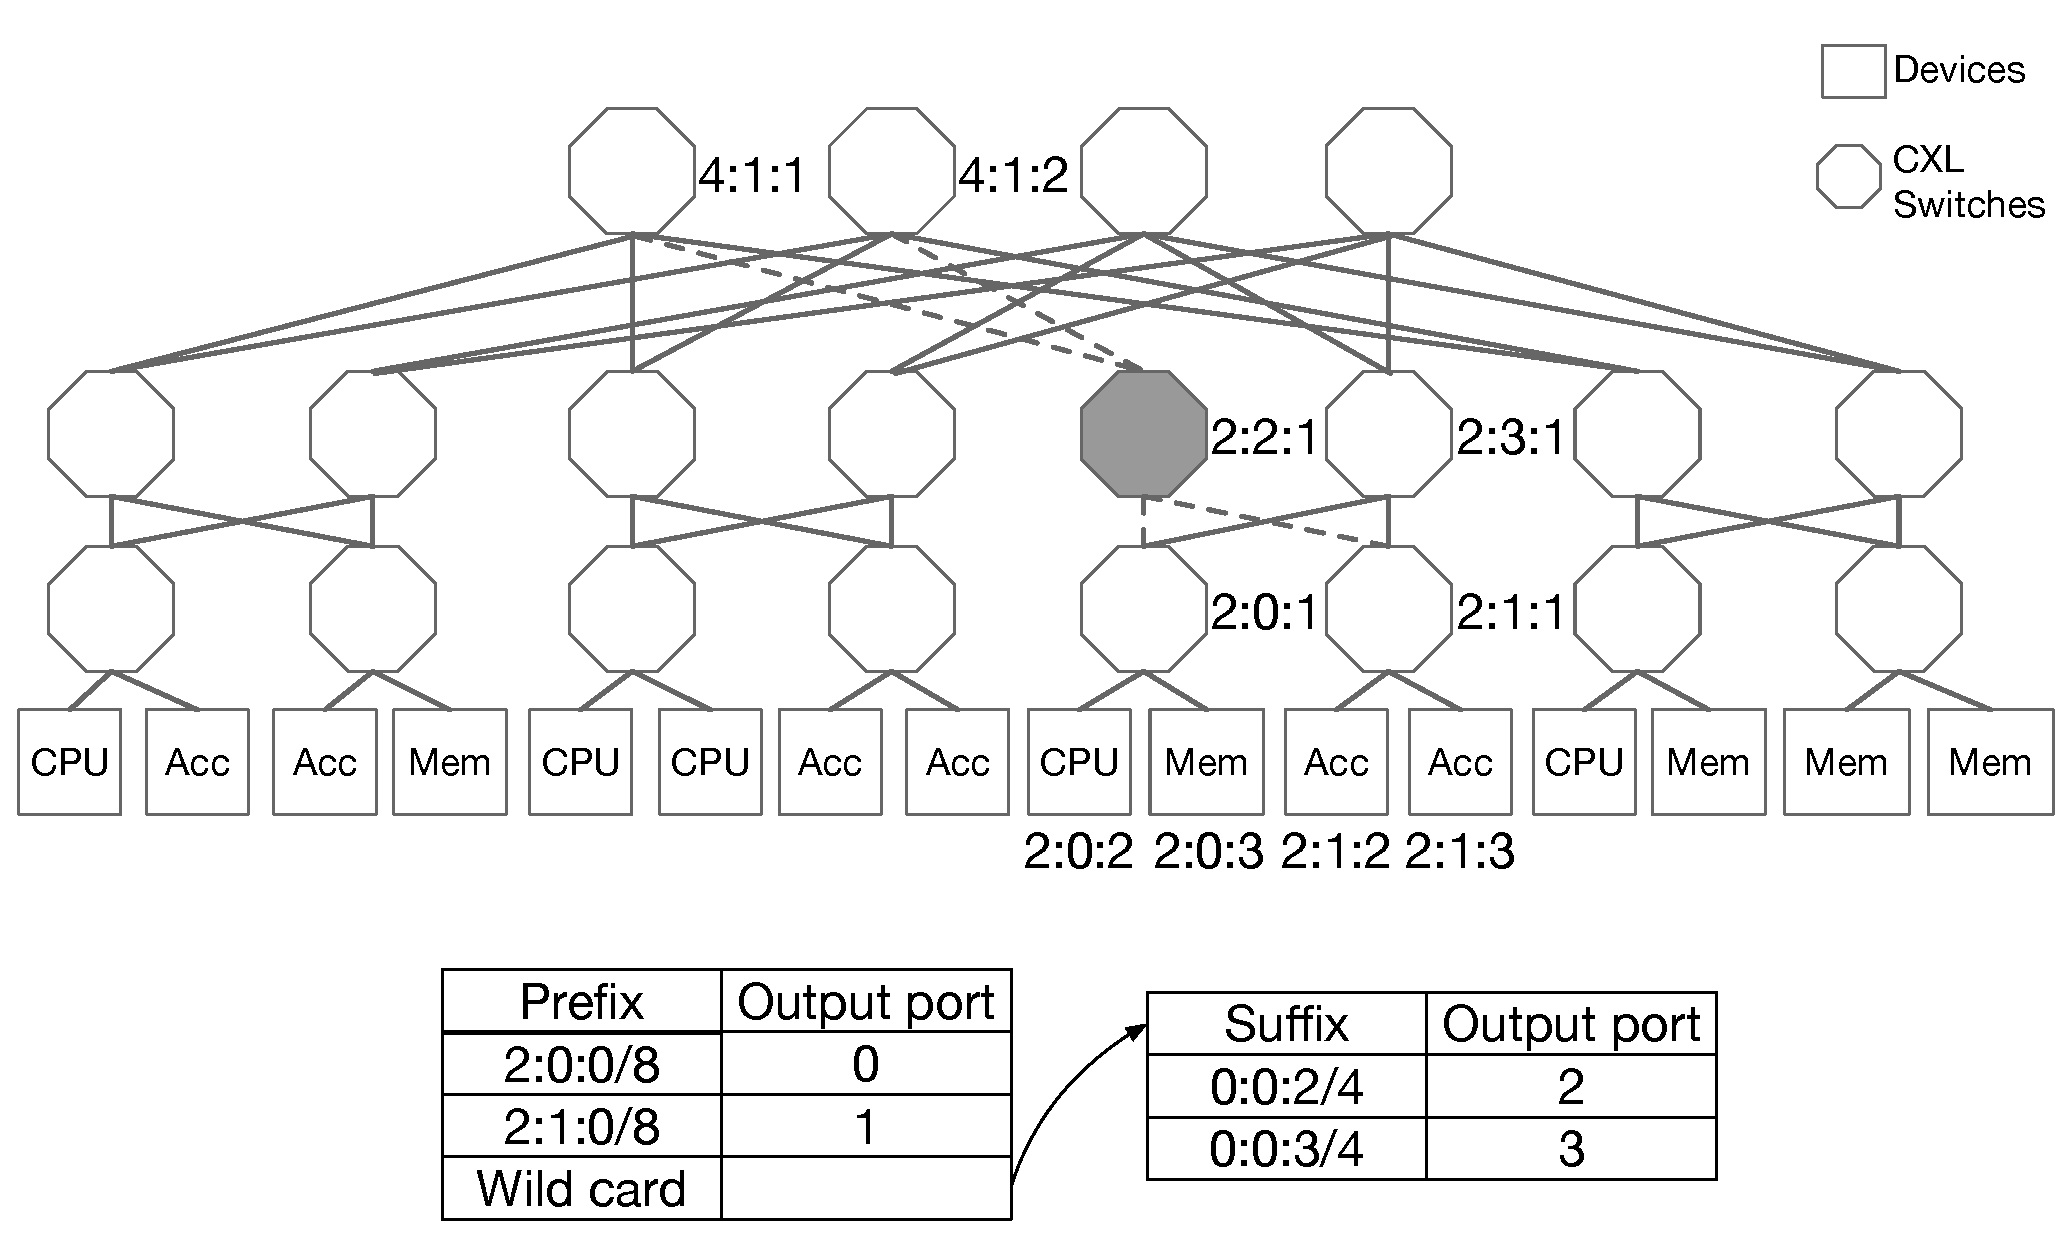
\includegraphics[width=0.9\columnwidth]{figure/aurelia/cxl-fat-tree-routing-table.eps}
    \caption{CXL fabric as a fat-tree using 12-bit FAN-ID address \emph{X:Y:Z}, which X, Y, and Z are hexadecimal values. Dash lines represent the routes from switch \emph{2:2:1}'s routing table.} 
    %representing \emph{pod:switch:device}}
    \label{fig:cxl-fabric-overview}
\end{figure}

We propose \aurelia, a network design involving devices and switches on the CXL fabric. 
%
\aurelia provides addressing, routing, and congestion control protocol design by augmenting necessary functionalities on the fabric interface and switches.
%
For the rest of Sec.~\ref{aurelia:sec:design} and further sections, non-oversubscribed fat-tree is assumed as the default topology to demonstrate the primitive addressing and routing design of \aurelia.
% 
% Fat-tree with oversubscription is out of the scope of this preliminary study. 
%
Different topologies with their related costs and configurations are discussed in Sec.~\ref{aurelia:sec:discussion}.

\subsection{Addressing \& Flow}
%
\aurelia proposes to generalize CXL's port ID scheme by assigning a 12-bit fabric node ID (FAN-ID) to a node that is either a device or a switch on the fabric. 
%
This is analogous to the 32-bit IP address describing hosts in an IP network.
%
%
FAN-ID assignment is agnostic to the underlying topology as long as a FAN-ID is unique for a node on a CXL fabric. 
%
% \aurelia assigns FAN-ID to the physical interface of the device. It does not assign FAN-ID to logical interfaces sharing the same physical interface.
%
%\aurelia considers multi-tenancy a device-specific detail and do not provide additional FAN-ID to logical CXL interfaces
%Multi-tenancy of devices is out of the scope of this work.

With a similar analogy to "5-tuple" in the IP network, \aurelia is able to defines a flow by a sequence of CXL packets that share the same source device, destination device, protocol, and message classes.
%
Thus, routable CXL packets can be identified with a quadruple: \emph{(Source FAN-ID, Destination FAN-ID, CXL protocol, message classes)}. The CXL protocols include CXL.io, CXL.mem, and CXL.cache. 
%
The message classes are subtype of packets within each protocol. 
%
For example, a CXL.mem packet writing to a device belongs to a class of \emph{M2S Request with Data} and a CXL.cache packet that carries responses from the device to the host belongs to a class of \emph{D2H Response with Data}.
%

% \begin{comment}
% %FAN-ID 
% %because routing design can be based on per-node FAN-ID
% %each device usually has a single CXL interface with potentially different number of lanes. 

% Also, given the limit size of 12-bit address space, it is not efficient to assign multiple addressses to a single switch. 

% Per port address design like MAC address is not necessary
% because \aurelia's routing design is modeled after IP level routing on switches. 

% dragonfly's routing
% Minimal (MIN) : The minimal path is taken as described in
% Section 4.1.
% Valiant (VAL) [32] : Randomized non-minimal routing as
% described in Section 4.1.
% Universal Globally-Adaptive Load-balanced [29] (UGALG, UGAL-L) UGAL chooses between MIN and VAL on a
% packet-by-packet basis to load-balance the network. The
% choice is made by using queue length and hop count to estimate network delay and choosing the path with minimum
% delay. We implement two versions of UGAL.
% UGAL-L – uses local queue information at the current
% router node
% \end{comment}

% \begin{figure}[htb]
%     \centering
%     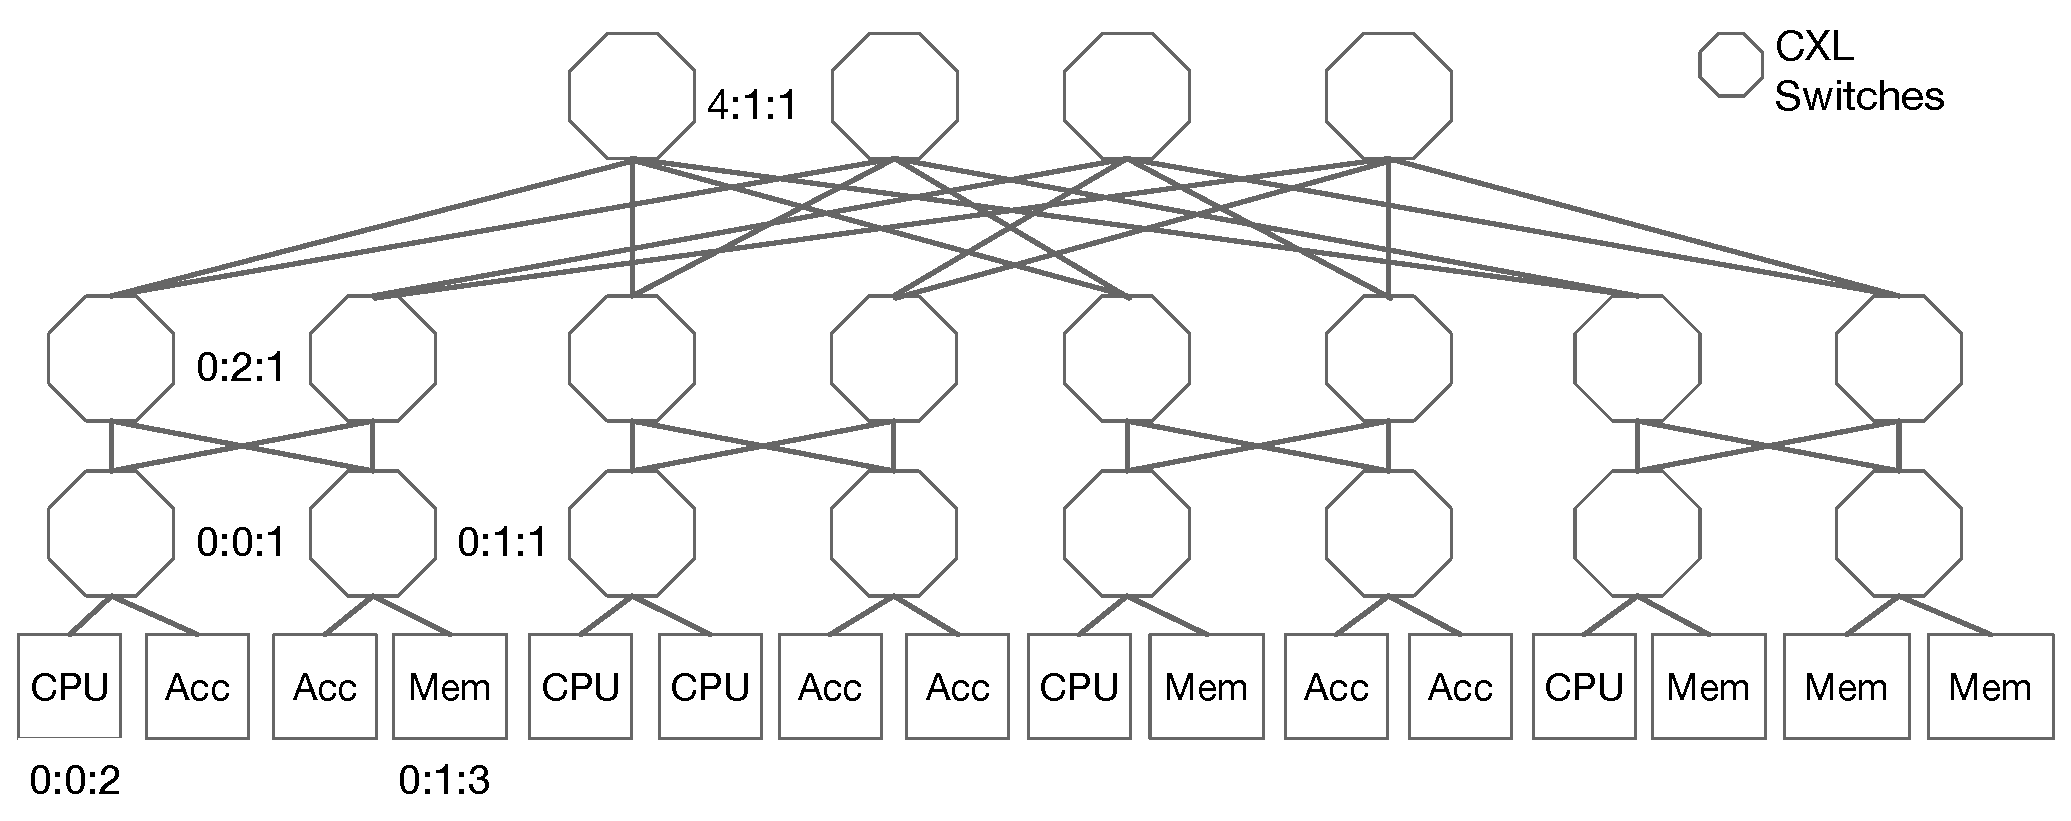
\includegraphics[width=\columnwidth]{figures/cxl-fat-tree-clear.eps}
%     \caption{\TODO{Routing example on Fat-tree.}} %representing \emph{pod:switch:device}}
%     \label{fig:fat-tree-routing}
% \end{figure}

\subsection{Routing}
\label{aurelia:sec:design:routing}
% P Path selection, R Routing itself, and L Load balancing. 
% Path selection determines which paths can be used for sending a given packet. Routing itself
% Routing answers a question on how the packet finds a way to its destination.
% Load balancing determines which path (out of identified alternatives) should be used for sending a packet to maximize performance and minimize congestion.
\aurelia routes packets based on FAN-ID addresses similar to IP routing.
%
CXL switches route a packet based on its routing table that maps a group of FAN-ID destinations onto a port. 
%
CXL switches transmit the packet out of a specific port to another switch that knows the next hop for this packet. 
%
The forwarding continues until the packet reaches the FAN-ID destination.

\noindent \textbf{Routing: Fat-tree as an example.}
%
Constructing a fat-tree~\cite{fat-tree:sigcomm:2008} with 12-bit FAN-ID address shows a $k$-ary fat-tree with $k=4$ in Figure~\ref{fig:cxl-fabric-overview}.
%
Fat-tree uses a hierarchical scheme that assigns FAN-ID to nodes as \emph{pod:switch:device} with three segments.
%
Each segment is a 4-bit hexadecimal value.  
%
For example, the leftmost CPU has FAN-ID \emph{2:0:2} representing it belongs to the third pod, the first switch, and the third node, which is right after the switch itself.
%
Similar to IP routing, the routing on fat-tree follows a single shortest path despite that the fat-tree topology provides path diversity.
%
This creates potential bottlenecks even for trivial communication patterns because of the underutilization of available bandwidth.
%
The fat-tree implements a two-level routing table on each switch. 
%
One level of the table routes traffic down to the device, while the other routes traffic toward the core of the fabric.
%
The table maps a set of destinations to a specific port. 
%
The table maps a set of destinations to a specific port. The routing lookup for destinations uses the address prefix for traffic downward to the devices and the address suffix for traffic going toward the cores.
%
The address suffix approach spreads traffic toward the fat-tree core across different switches based on FAN-ID.
%
The bottom of Figure~\ref{fig:cxl-fabric-overview} shows the routing table of CXL switch \emph{2:2:1} filled in gray.
%
The prefix table routes packets toward its downstream switches \emph{2:0:1} and \emph{2:1:1}. 
%
The suffix table routes the packet upward to core switches \emph{4:1:1} and \emph{4:1:2}.  
%\TODO{add a running example on to Figure~\ref{fig:fat-tree-routing} or a new one.}
%

% \begin{comment}
% After identifying the quadruple, the existing knowledge of using flow as a major abstraction of load balancing and optimization becomes applicable for CXL fabric flow~\cite{FlowBender, Hedera, MicroTE}. In the case of multi-tenant devices, the quadruple cannot distinguish traffic between different tenants. Thus, per-packet load balancing schemes are more applicable for multi-tenant scenarios~\cite{Fastpass, DeTail, MPTCP}. 

% \weitao{Since we already assume next-generation connection, do we want to mention that the fat-tree topology can be a baseline, and we could further optimize the topology based on the application traffic pattern, like adding more number of lanes between frequently communicated devices.} 
% \stingw{I agree. topological optimization is a nice direction but it's hard to do it with current or near-future CXL technology. We can put it to the Discussion.}
% \stingw{We'll need CXL with higher radix to have more exotic topology, e.g. Dragonfly, Jellyfish, Xpander}

% \weitao{Active routing is another interesting type of routing. It is developed based on load-balancing routing. When one path is congested for a substantial amount of time, some flows will change the flow label to change the 5-tuple, so that the flow will pick a new path automatically. In your case, do you think you can also add a similar thing in "5-tuple" to make it "6-tuple" and enable active routing?} \stingw{introducing additional things on CXL's 256-byte packet is hard given the limited space. I don't agree with this one.}
% \end{comment}

% \TODO{we should talk about how the fabric manager will be implemented. GPU-SSD example is not a good one.}
% \reviwer{B: I encourage you to be more explicit about what's in/out of scope for the fabric manager}
%mirador:fast:2017, 
%uses multiple devices together~\cite{gullfoss:tech-report:2015, fractos:eurosys:2022}.
%
% \stingw{take out the GPU example!}
% The GPU-SSD example in Sec~\ref{sec:motivation:routing} is exactly one of these workloads.
% %
% The detouring of peer-to-peer memory access to an additional hop of memory buffer is not trivial to be specified as routing rules. 
% %
% The fabric manager first determines a fabric-attached memory device as the destination, then redirect the routing between the producer and the consumer devices to the memory device instead.  
% %
% The fabric manager then asks the consumer to read from the specific memory device instead of directly communicating with the producer.

\noindent \textbf{Multi-path routing.}
%
The two-level routing table of the fat-tree is an implementation of multi-path routing tailored to a specific topology. 
%
\aurelia imposes no restriction on how the fabric should be constructed. 
%
Instead, \aurelia is able to have routing tables that map a destination to multiple next-hop FAN-ID and its corresponding metric. 
%
These metrics can include distances in terms of hops or local congestion level on each switch port. 
%
\aurelia selects a next-hop with minimal metric and randomly selects one if there are multiple next-hop options with equal metrics.  
%
Considering the number of hops for shortest path routing, \aurelia can perform a random selection for the next hop on flow granularity or on packet granularity, i.e. Equal-Cost Multi-pathing (ECMP), or at the packet granularity, similar to packet spraying.

\noindent \textbf{Adaptive routing.}
%
ECMP and packet spraying are oblivious to the workload. 
%
\aurelia is able to to achieve adaptive routin by further exploiting local per-port information on the switches or by manipulating the routing table on the fabric manager.
%
\aurelia uses per-port EP Backpressure as a measure of local congestion. 
%
For selecting an egress port with minimal congestion on the switch, \aurelia uses power-of-2 choice~\cite{power-of-two:tpds:2001} to avoid congestion on ports based on possibly delayed congestion information.
%
Additionally, \aurelia allows the fabric manager to insert routes and has the sole authority to modify the routing table at any time.
%
This is useful for the workload that requires non-trivial routing tailored to specific workloads~\cite{gullfoss:tech-report:2015, fractos:eurosys:2022}. 

\begin{figure}[ht!]
    \centering
    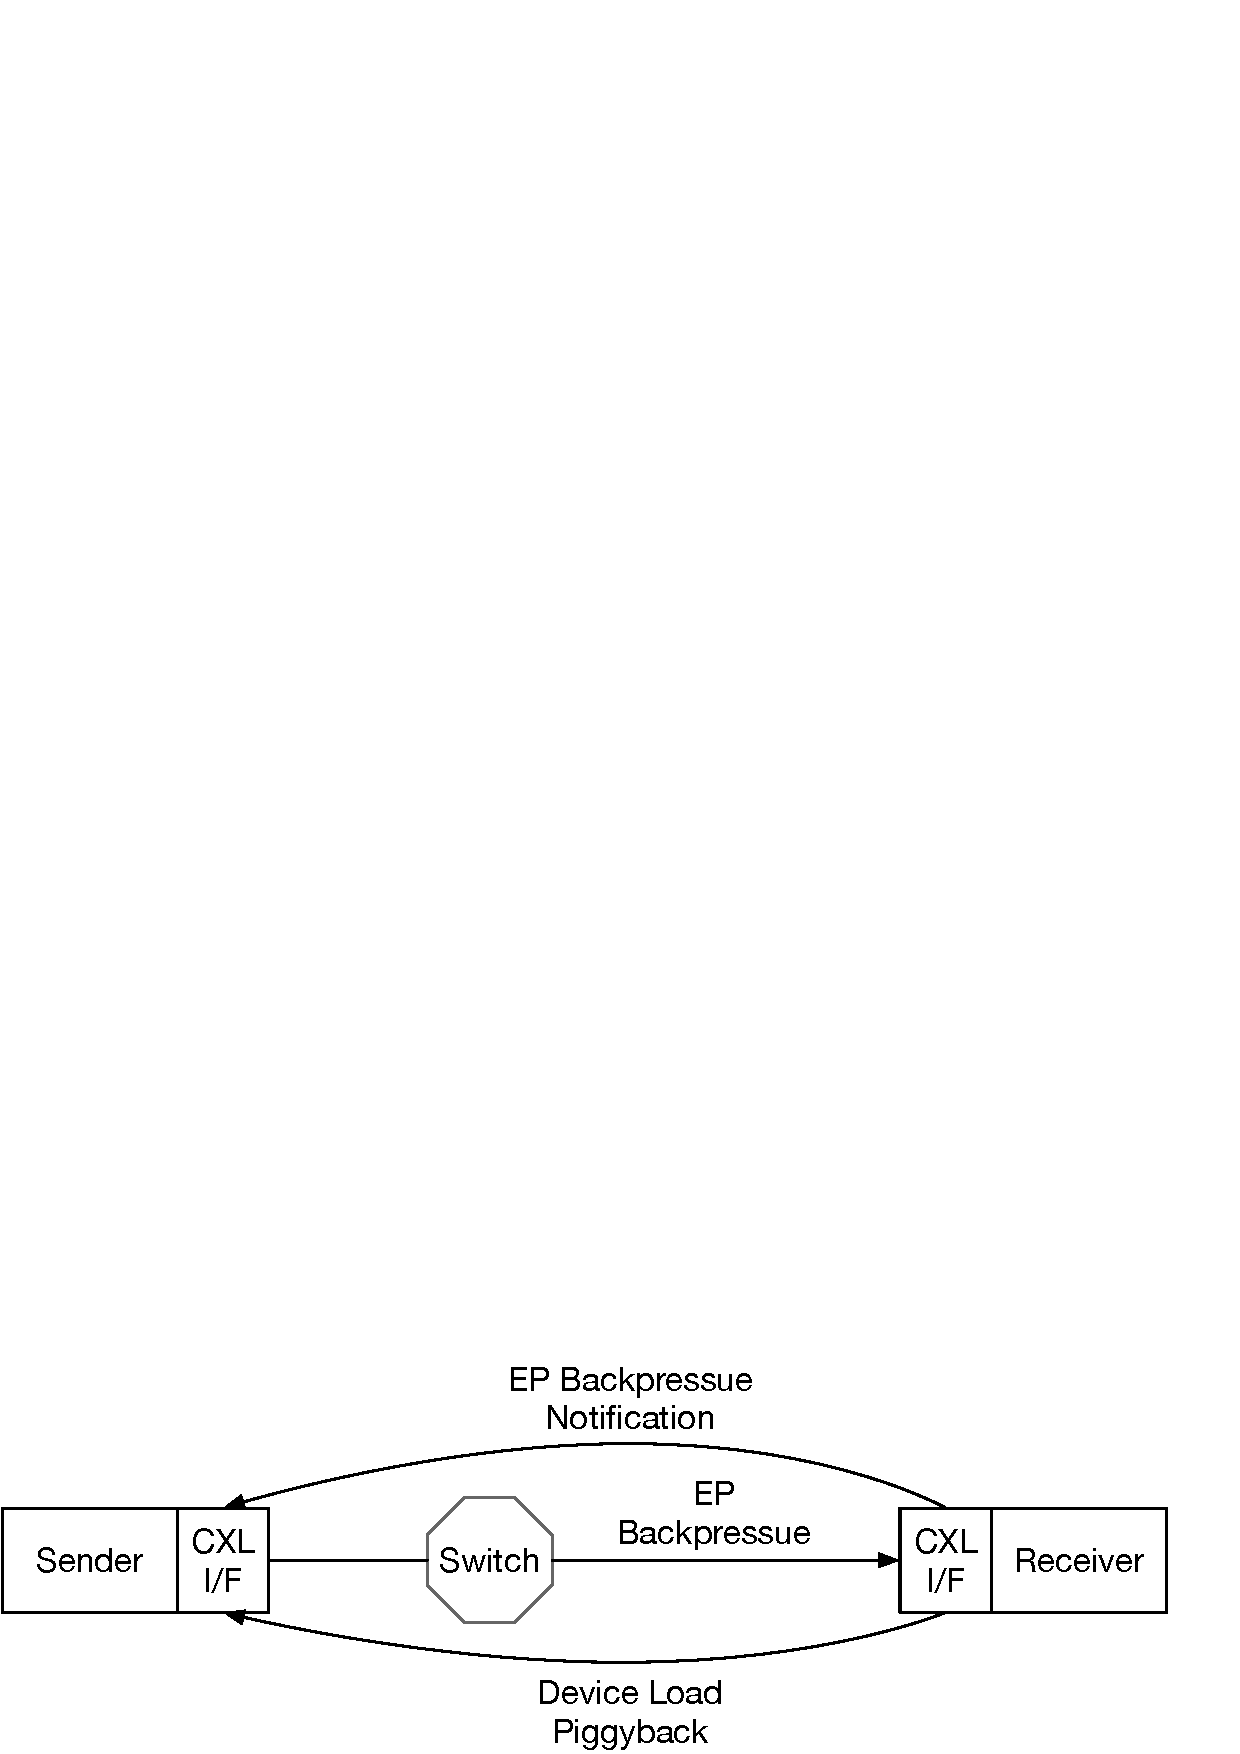
\includegraphics[width=0.9\columnwidth]{figure/aurelia/congestion-control-flow.pdf}
    \caption{\aurelia uses EP Backpressure notification to resolve congestions and overload signal for flow control to avoid overrunning the buffer on the device.}
    %has a congestion control loop for the fabric, a flow-control loop for the device.}
    \label{fig:congestion-control}
\end{figure}

\subsection{End-to-end Congestion Control}
\label{aurelia:sec:design:congestion-control}
%\TODO{Steve: You need an introductor paragraph before the bolded paragraph.}

CXL relies on point-to-point flow control that is prone to congestion and lacks a congestion control design for the fabric.
%
As stated in Sec.~\ref{aurelia:sec:motivation:transport}, CXL's QoS telemetry and EP Backpressure partially mitigate congestion for specific scenarios.

QoS telemetry currently supports only CXL.mem protocol between the host and devices with their locally attached memory.
%
QoS telemetry enables memory devices to indicate their current internal load with 2 bits for CXL.mem response packets.
%
The sender on the host CPU uses this reported internal load to monitor and throttle its request rate. 
%
However, not every sender on CXL fabric is on the host CPU. 
%
Peer-to-peer memory accesses using Unordered I/O of CXL.io allow devices to access the memory of another device directly. 
%
These peer-to-peer accesses under CXL.io are not throttled in the current design because QoS telemetry is limited to CXL.mem and does not consider the sender to be other than a host CPU.
%

EP Backpressure is not effectively utilized in the current design of QoS telemetry, because QoS telemetry determines the overall load of a device by taking the maximum of the device's internal load and EP Backpressure. 
%
This approach subsumes EP Backpressure that offers valuable congestion information on the fabric.
%
By simply taking the maximum value of the separated piece of information, QoS telemetry provides neither accurate device internal load nor congestion on the fabric.
%
This inaccuracy hinders QoS telemetry's ability to perform effective end-to-end flow control and congestion control for the transport protocol. 
%
The aforementioned challenges motivate us to design \aurelia.

% \stingw{More on pointing out the unique challenge, don't argue against delay based approach too much. Stay neutral before we have strong evidence.}
% \balance
% \begin{comment}
% These devices have shallow buffer space and different rate of producing/consuming data. %and are allocated with different bandwidth on the fabric.
% %
% With strictly peer-to-peer communication, the producer matches consumer's rate to not overwhelm the consumer. 
% %
% The slow-down on faster producer leads to under-utilization of the device. 
% %
% To improve resource utilization, fabric attached memory pool can serve as the buffer and an alternative routing destination between devices. 
% %
% This decouples the producer and the consumer and allows faster producer to be utilized by other workload.
% %
% The switch identifies CXL.io packets performing peer-to-peer memory access, and notifies the fabric manager when it sees EP Backpressure on its port with CXL.io.
% %
% The fabric manager modifies the routing table between the producer and consumer, and routes the packets to a specific fabric attached memory pool attached to the either side of the CXL switch. 
% %
% The fabric manager then asks the consumer to read from the specific fabric attached memory pool instead of directly communicating with the producer.

% \weitao{One suggestion about the signals: the internal load and the EP backpressure could be represented in a uniform format. Both of them suggest the congestion level, but for end-point devices and switches respectively.}\stingw{this sounds about right!}

% \weitao{Another wild idea is that, if switches and end-point devices could provide more quantitative signals (like 8 bits) to represent congestion level, rather than a single bit to provide a binary signal about congestion, the performance of the congestion control algorithms could be largely improved. As a supporting fact, many commodity switches can support reporting and piggybacking telemetry information for each packet, including per-hop queueing delay and per-hop utilization.}\stingw{the problem with CXL is the packet is 256-byte. we could argue for using more bits in the discussion section. I tried to do the minimal modification to CXL to achieve something useful.}    
% \end{comment}
\noindent \textbf{Extending existing mechanisms.}
%
\aurelia implements end-to-end congestion control with overload avoidance by extending the existing mechanisms of CXL. 
%
The mechanisms are EP Backpressure on switches, internal load reported on receiving devices, and rate throttling on sending devices.
%
%EP Backpressure and ECN both indicate congestion explicitly to the receiving endpoints.  
%and need packets to convoy the congestion signal back to the sender.
%
EP Backpressure triggers switches to mark packets on their way to the receiving device when noticeable queuing occurs on the switch.  
%
This is similar to Explicit Congestion Notification (ECN) for Ethernet and Infiniband because they react when the queuing situation begins to indicate congestion.
%
Internal load reporting triggers an overloading signal when the device is overloaded. 
%
Device overload is likely to cause significant device-side delay or even loss of CXL packets.
%
\aurelia, unlike CXL's design, separates EP Backpressure and the device's internal load since they represent fabric and device information. 
%
% for congestion control and overload avoidance 
% EP Backpressure and internal load use 1 bit for each on the packet header. 
%
Rate throttling controls the sending rate into the fabric to avoid congestion and overload. 
%
%On top of these mechanisms, CXL fabric is a lossless fabric by its point-to-point flow control design.
%
% These factors determine \aurelia to implement a rate-based congestion control with overload avoidance for the devices. 

\noindent \textbf{Algorithm.}
\aurelia's congestion control algorithm operates on the switch, the receiving device, and the sending device.
%
On the switches, \aurelia mandates the switches to mark the packets when the ratio of EP Backpressure events in their recent window is larger than a specific threshold.
%
On the receiving devices, \aurelia makes the receivers piggyback an overloading signal to the sending device when its sending rate exceeds the receiver's processing rate.
%
The receiving device notifies the sender with EP Backpressure notification (EPN) in its response to the sending device when it receives EP Backpressure marked packets. 
%
On the sender side, the sending device throttles the sending rate based on the 1-bit signal of EPN and the 1-bit overloading signal. 
%
When the sender receives a response packet marked with EPN or an overloading signal, the sender records its current rate $R_{c}$ as the target rate $R_{t}$ for later recovery and cuts its rate half by default. 
%
The rate cut can also be determined by also a rate reduction factor $\alpha$, similar to DCTCP and DCQCN~\cite{dcqcn:sigcomm:2015}.   
%
The recovery of the reduced sending rate has two different paths depending on the trigger.
%
If the reduction is triggered by EPN, then the recovery to the target rate $R_{t}$ is expected in a fixed number of iterations. 
%  
If the reduction is triggered by an overloading signal, then the recovery is an additive increase.

% \stingw{fast recovery for EP Backpressure and slower recovery, i.e. additive, for internal load}
%
% \stingw{EP Backpressure and internal load use 1 bit for each on the packet header.}

%Flow control preventing buffer-overrun is handled by the link and physical layer of CXL and thus not a concern for the transport layer. 

\noindent \textbf{Protocol implementation.}
\aurelia relies on hardware implementation to throttle sending rate for congestion control due to sub-$\mu$s latency and peer-to-peer memory access requirements.
%
First, rate throttling has a tight latency requirement of sub-$\mu$s on CXL fabric.
%
Pond measured end-to-end CXL.mem latency and obtained latency ranging up to 270 ns on CXL system with a single switch~\cite{cxl:hoti:2022, pond:asplos:2023}. 
%
Under the same assumption, the latency of CXL packet traveling through a two-level fat-tree takes around 680 ns, which is under 1 $\mu$s.
%
Second, peer-to-peer memory access between devices is expected, especially with the usage of accelerators. 
%
Therefore, \aurelia extends CXL's original design to generalize the reporting of device load for all kinds of memory access, including peer-to-peer memory access between devices.
%
Peer-to-peer memory access between devices without an additional embedded CPU motivates the necessity of implementing rate throttling in hardware on the CXL interface. 
%
The control plane of these hardware devices is kept on the host CPU, but the execution of rate throttling is on hardware to meet these requirements.  
%
Hardware-based rate throttling ensures all devices on the CXL fabric are able to control their sending rate and further reduces the congestion and overload.
%
Implementing rate throttling logic on hardware has been used on RDMA over Infiniband and Ethernet with RoCEv2 support and thus suggests the feasibility in the case of CXL fabric. 

\noindent \textbf{Comparable protocol design on lossless fabric.}
\aurelia's congestion control design is inspired by congestion control on existing lossless fabric, such as Infiniband and DCQCN for RoCEv2, which implemented a rate-based congestion control algorithm requiring Explicit Congestion Notification (ECN) on switch to indicate congestion.
%
Infiniband switches mark packets with a Forward ECN (FECN) bit when congestion is detected~\cite{infiniband-spec}. 
%
The receiver receives the FECN-marked packets and sends a Backward ECN (BECN) marked packet to the sender.
% 
The sender throttles its injection rate when it gets packets with BECN. The throttling over time reduces congestion and the fabric returns to a state without any congestion. 
%
The FECN marking of packets requires switch support and the implementation of BECN and rate throttling requires additional logic in CXL interface hardware.
%
DCQCN, a congestion control protocol designed for RoCEv2, relies on the ECN of Ethernet to notify the sender to adjust its injection rate, similar to Infiniband~\cite{dcqcn:sigcomm:2015}.
%
% Before throttling, \aurelia sets the rate as the target rate for later recovery.
% %
% \aurelia throttles the rate of the sender, when the receiver notifies it of the congestion signal and generates EP Backpressure. 
% %
% After rate throttling, \aurelia enters the recovery phase and then performs additive increase when approaching the target rate~\cite{dcqcn:sigcomm:2015}.

\section{Evaluation of \aurelia's Design}
\label{aurelia:sec:eval}
%
We simulate the design of \aurelia because CXL hardware supporting CXL 3.0 with fabric is not available to the author at the time of writing.
%
We evaluate \aurelia's congestion control design using routing described in Sec.~\ref{aurelia:sec:design:routing}. 
%
Additional routing designs, such as multipath and adaptive routing, are not enabled for the evaluation.
%
The evaluated workloads are: (1) key-value store on memory expansion modules~\cite{samsung-memory-expander:hcs:2022}, and (2) machine learning model inference on GPUs/accelerators involving collective communication~\cite{aws-inferentia:2019}.
%
They represent different uses of CXL fabric: one focuses on CPU and memory expansion, while the other focuses on the data exchange between accelerators.
%
The baseline of the evaluation is vanilla CXL described in its specification~\cite{cxl-3-0-spec}.
%
It performs point-to-point flow control for packets of each CXL protocol.
%
It does not employ any end-to-end congestion control or flow control mechanisms.
%
% \stingw{It has limited support for dev load reporting for CXL.mem
% but it does not consider the fabric situation.}

% \TODO{Define the baseline here please.}
% \stingw{
% What are we comparing to?
% %
% CXL default with only PCIe flow control.
% %
% Make sure the large flows don't shut down the port if flows collides.
% }
%\stingw{The issue with PCIe is that all traffic are fighting together. CXL-base has different protocol and message classes}  

\subsection{Packet-level Simulation using ns-3}
\label{aurelia:sec:eval:ns3-simulation}
We use NS3~\cite{ns-3} to simulate packet level behavior on a CXL fabric.
%  
NS3 is a discrete-event network simulator that is open-sourced and well-established in the research community. 
%
Our implementation uses primitive, built-in NS3 classes and starts from scratch because there is no existing simulator for the CXL fabric. 
%
Previous simulators of other lossless fabrics focus on RDMA over Converged Ethernet (RoCE)~\cite{dcqcn:sigcomm:2015, hpcc:sigcomm:2019,pint:sigcomm:2020}.
%
These implementations are not usable for CXL fabrics because they assume the use of Ethernet, IP, and the RDMA interface cards.
%
CXL fabrics assume none of those, as the devices on the fabric issue load/store instructions directly.   
%
%The difference between our simulation and the latencies reported on the CXL expansion chassis is within 5\%.

The hardware parameters are cross-checked with published literature~\cite{pond:asplos:2023, demystifying-cxl:micro:2023, h3platform-cxl-memory}. 
%
The latencies on each hardware component are calibrated with H3 platform's CXL expansion chassis supporting CXL 2.0~\cite{h3platform-cxl-memory}. 
%
The chassis integrates a CXL switch~\cite{xconn-cxl2-switch} supporting CXL.mem and CXL.io that are used in the evaluation.

We simulate CXL's transaction layer and link layer in 256B mode assuming a PCIe 6.0 physical layer.
%with its forward error correction are fully controlled by the hardware.     
%
The physical layer of PCIe 6.0 with 256 GB/s is on a 16-lane configuration. 
%
All links in the simulation use this configuration.
%
All messages classes of CXL.mem and CXL.cache are supported.  
%
CXL.io functionalities for peer-to-peer memory access are supported. 
%
Packing of CXL.mem and CXL.cache messages is implemented to ensure the number of packets on the fabric is accurate to the specification.

The simulator enables multi-level switching and implements \aurelia's addressing, routing, and congestion control mechanism on top of CXL's port-based routing.
%
There are 16 nodes on a 2-level fat-tree topology. 
%
In the case of machine learning model inference, the topology connects 8 accelerators and 8 memory expansion devices.
%
In the case of the key-value store, the topology connects 12 memory expansion devices with 4 CPUs.
  
%
\subsection{Simulation of Large Model Inference}
\label{aurelia:sec:eval:inf}
%
We study the improvement of inference throughput on the LLaMA2 70B model~\cite{llama:arxiv:2023} due to improved congestion control on the CXL fabric.
%
The inference of the model operates on the unit of tokens for a sequence of input and output data.
%
First, the fabric connects the accelerators to the memory expansion devices that store the model weights.
%
Partial weights of the model are kept on the accelerator as the weights are loaded partition by partition.  
%from the memory expansion devices.
%
Each accelerator stores an 8.125 GB partition on the device and another partition on the memory expansion devices.
% The weight loading and inference exec are pipeline parallel.
%
This leaves enough capacity for intermediate generated tokens on the accelerators.
%
A run of inference performs 2 weight loading operations between the accelerators and the memory expansion devices.
%
Second, the fabric supports the communication among accelerators that aggregates tokens.
%
A run of inference performs 2 operations of all-reduce collective communication among the accelerators to aggregate the intermediate and the output tokens.
%
Each all-reduce operation exchanges 810 $\times$ 8 MB of data among the accelerators.
%
The all-reduce operations are 3 milliseconds apart as these durations represent the computational part of the inference run.
%
The simulation executes 1000 runs of inference based on the aforementioned parameters.  
%
\aurelia's improved congestion control aims to speed up both the weight loading and the all-reduce operations.
%
% The 3 milliseconds durations corresponds to the two major components of the LLaMA2 model, self-attention and feedforward layers.    
% These tokens are an $E$-dimensional vector, where $E$ is 16384 in our setup.
% %
% A sequence has up to $L$ tokens, where $L$ is 256 in our setup.
% %
% A run of inference processes $B$ $L$-token sequences containing $E$-dimensional vectors, where $B$ is the batch size of 2048 in our setup.

\aurelia achieves 21\% improvement on median throughput and 27\% improvement on the 10th percentile throughput because of faster weight loading and all-reduce operations.
%
These operations encounter 2.1$\times$ fewer pauses on the links than the baseline when the links are out of credits to send packets.
%
EPN of \aurelia throttles the sending rate to avoid triggering pauses on links. 
%
The traffic pattern of weight loading and all-reduce operations does not create much imbalance therefore there is no overload on any of the accelerators that requires an overload signal for remediation.
%
Imbalanced traffic among accelerators could test \aurelia's effectiveness on such kind of traffic pattern. 
%
We leave it for future investigation.

\subsection{Simulation Results on YCSB Benchmarks}
\label{aurelia:sec:eval:kv-store}
%\TODO{Using A, B, C, and F results with ns-3 simulation}
%
We study the 99th percentile latency on key-value stores using YCSB benchmarks \cite{ycsb:socc:2010}.
%
YCSB benchmarks are widely used to evaluate key-value stores with a mix of insert, read, and update operations in memory or on SSD.
%
%They are used to evaluating key-value stores in memory or on SSD.
%
In the case of CXL fabric, we evaluate key-value stores on fabric-attached memory expansion.
%
Memory expansion devices manage their own coherence between themselves and connected CPUs.
%
They invalidate data in the CPU cache to maintain the coherency.

%\stingw{why scan operations are not doable in our setup, so we only do A, B, C and F.}
We evaluate YCSB A, B, C, and F for read, write, and read-modify-write operations on the key-value store.
% insert is weak here. 
%
YCSB D and E are not evaluated because their performance depends on the recently accessed keys and also how the keys are hashed when inserted. 
%
These additional requirements make them less ideal for us to objectively evaluate the improvement provided by \aurelia.
%
YCSB A, B, C, and F, on the other hand, access key-value pairs based on a fixed Zipf distribution.
%
The Zipf distribution makes the probability of accessing $n^{th}$ key inversely proportional to $n$.
%
The plot of a Zipf distribution in linear scale is similar to an exponential decay curve so the first few $n^{th}$ keys are way more likely to be frequently accessed.
%
This makes the traffic imbalanced because the requests to a key-value pair are more likely to be headed to a certain memory expansion device. 

% \stingw{
% %For D: Request distribution: latest, E needs scanning for a range. 
% For D, it needs an assumption of the latest and assumes inserts are hashed. 
% Therefore, its performance depends on the hash for the "latest" distribution.
% %
% For E, scanning also depends on the hash for insert. 
% %
% This hash heavily impacts how the performance will be looked like and it's not a fixed distribution like Zipf we can control. 
% }

\begin{figure}[ht!]    
    \centering
    \includegraphics[width=0.9\columnwidth]{figure/aurelia/ycsb.pdf}
    \caption{YCSB benchmarks with higher ratio of writes demonstrate more improvement.} 
    \label{fig:cxl-ycsb-results}
\end{figure}

\aurelia's improvement on 99th percentile latency for YCSB benchmarks is shown in Figure~\ref{fig:cxl-ycsb-results}.
%
\aurelia's EPN and overload signal combined handle the imbalance of traffic caused by Zipf distribution. 
%
The improvement for read-only YCSB C is the lowest because it incurs a request-response pair to a specific memory expansion device without any cache invalidation.
%
The improvement for YCSB A and B is higher because YCSB A and B incur write and subsequent cache invalidation from the memory expansion device to other CPUs.
%
The improvement of YCSB A is higher than YCSB B because it has 50\% of operations as writes operations compared to 5\% of YCSB B.  
%
EPN has a higher contribution to the latency improvement because 
the overload signal contributes 22\% more improvement on YCSB F compared to \aurelia without it.
%
This is expected as overload should not be a frequent event unless memory capacity and bandwidth are not properly provisioned
%
On average, \aurelia without overload signal is only 14\% worse on all YCSB benchmarks.

% \stingw{The explanation: EPN handles the congestion and overload signal in this case does contribute to it.
% %
% But I guess the question is about the ratio? 
% %
% 22\% more on YCSB F compared to \aurelia without it. In average, 14\% more on all.
% }
%
%\TODO{A figure for 99th percentile latency on YCSB A, B, C and F.}

%\section{Additional Fabric Enhancement Consideration}
\section{Discussion}
\label{aurelia:sec:discussion}

\aurelia demonstrates a fabric for disaggregation based on the CXL specification~\cite{cxl-3-0-spec}. 
%
However, CXL is not the panacea for every issue and challenge in the dataceneters. 
%
First, 
alternative fabrics like NVLink for GPUs and PCIe for existing devices are discussed with their advantages over CXL.
% 
Second, CXL is limited to a shorter range of reach compared to Ethernet.
%
With CXL's limitation in the physical layer from PCIe, Ethernet is still much needed for inter-rack communication.
%
Third, CXL fabric flexibility on topology motivates us to discuss multi-pathing strategy based on specific topologies.
%
Lastly, CXL externalizes system interconnect to connect more devices than ever and thus further exposes itself to more potential side-channel attacks

%\TODO{Steve: You need an introductor paragraph before the bolded paragraph.}
%\TODO{extending discussion for 6-page HotNets}
% \noindent \textbf{The scale and economic of CXL fabric}
% how large should we scale CXL fabric to be still cost-effective~\cite{pond:asplos:2023}?
% Pond dem
\noindent \textbf{Alternatives: NVLink and PCIe fabric.}
%\TODO{Clean up the text here!}
% \stingw{Here to add NVLink + GH-200 discussion. 
% NVLink is propriety and has a narrower usage even with GH-200.
% GH-200 with NVLink is at most a CXL type-2 usage.
% }
%\stingw{All these alternatives are not designed to be as general as CXL}
%
% Alternative interconnects are designed for specific use cases, and they lack of the generality of CXL. 
% 
NVLink is an interconnect by Nvidia for high throughput between GPUs~\cite{nvlink}. NVLink supports GPU-CPU interconnect with cache coherency on the recent Grace-Hopper 200 hardware~\cite{dgx-gh200}. 
%
NVLink presents an interesting alternative to CXL but has three limitations. 
%
First, GPUs using NVLink with cache coherence are equivalent to CXL type 2 devices. 
%
However, NVLink does not support CXL type 3 devices, which expand memory independently of the main memory capacity.
%
The capability to scale memory capacity is attractive for memory-hungry large language models~\cite{gpt3:neurips:2020,llama:arxiv:2023}. 
%%NVLink with its cache coherent extension presents an alternative of CXL Type2 interconnect.   
%
Second, NVLink scales to 256 endpoints but connects only GPUs as endpoints~\cite{dgx-superpod}. 
%\stingw{Third, NVLink itself does not scale beyond 8 or 16 GPUs on a server.}
Third, NVLink as a proprietary interconnect limits its usage beyond Nvidia's hardware.
%
PCIe using Non-Transparent Bridge (NTB) expands beyond a single root complex to multiple hosts as a fabric with many more connected devices~\cite{pcie-spec}. 
%
%PCIe transactions mapped to NTB’s specific memory range are forwarded
%with address translation to the destination host.   
%
% Using NTB with a shared address space spanning all hosts and their devices enables devices to directly communicate with point-to-point DMA over PCIe fabric~\cite{gigaio-fabrex}.
%
However, PCIe, included in CXL as CXL.io, lacks the memory and caching semantics that are much needed in the face of accelerators and memory expansion. 
%
This is exactly the reason that motivates the creation of CXL.
%
Both NVLink and PCIe fabric support a subset of CXL's use cases but do not support all of them.
%
%\stingw{why not hooking Ethernet directly to each device?}

\noindent \textbf{Co-existence of CXL and Ethernet.}
Given the scaling discussion, CXL is still unlikely to completely replace Ethernet in the datacenter due to its current PCIe based physical layer design. 
%
We speculate CXL fabric is beneficial on a rack-scale due to its signal integrity and CXL switch hardware cost.
%
CXL fabric is not intended to replace existing Ethernet completely but to be a cost-effective alternative at the rack level. 
%
CXL packets are converted to Ethernet frames at a location equivalent to a top-of-rack switch for cross-rack traffic.
%
Previous work investigating the co-existence of Ethernet and a memory fabric follows a similar approach~\cite{aquila:nsdi:2022}.

%\stingw{Interconnect comparison: NVLink + C2C, other inter core interconnect, PCIe, CXL}
\noindent \textbf{Cost-effective scales of CXL fabric:}
%\noindent \textbf{Co-existence of CXL and Ethernet.}
% \stingw{how large should we scale CXL fabric to be still cost-effective~\cite{pond:asplos:2023}?}
%
CXL is an exciting technology, but it comes with its limitations.
%
First, CXL requires a retimer to maintain its signal integrity after a 500 mm distance~\cite{microchip-cxl-retimer,asteralabs-pcie-retimer}. The retimer raises the hardware cost and incurs an extra 20 ns latency every 500 mm~\cite{pond:asplos:2023}.
%
Second, to scale CXL supporting multi-level switching, multiple CXL switches are used. They cause an estimated 70 ns latency for each hop over a switch.
%
Considering the combined cost of switches, retimers, and additional memory controllers, Pond~\cite{pond-saving:ieee-micro:2023} suggests a scale smaller than 32-socket for their memory expansion usage (shown in Figure~\ref{fig:kvs-cxl}).
%
However, the exact scale of cost-effective CXL fabric for model training and HPC usage (shown in Figure~\ref{fig:ml-acc-cxl}) remains to be determined in future work.
%
%Pond also suggests the exact scale of a cost-effective CXL fabric depends highly on the workload, e.g. Pond's memory expansion usage for VM on public cloud.

% \stingw{CXL is not a solution for everything. It has signal integrity limits that making it scale beyond not cost-effective and with bloated latency by these intermediate retimers and switches.}
%
% \stingw{Pond suggest 8-socket for the use case is shown as Figure 1-(b). Pond also said that the exact scale depends on the workload. If the workload can tolerate higher latency or has a clear and predictable memory access pattern, then the scale of CXL can be larger if it's cost-effective.}
%    

\noindent \textbf{Topologies and multipathing.}
The flexible topology of CXL fabric empowers the fabric operator to optimize their topology based on 
their cost consideration and traffic pattern.
%
Though fat-tree offers straightforward addressing and routing, it requires many switches and incurs high wiring costs. 
%
Topologies require fewer switches and less wiring, e.g. 
Dragonfly or other low-diameter alternatives, could be considered if cost is the primary concern.
%
The recently released CXL 3.1 supports native multipathing. 
%
Topologies with high path diversity, such as Dragonfly, can be easily implemented with CXL's multipathing. 
%
Packet spraying and ECMP on fat-tree-related topologies can benefit from this as well.
%
With CXL switch prototype supporting 32 ports~\cite{xconn-cxl2-switch}, we expect these higher radix switches to enable more design options.
%
For example, the fabric operator can assign a high over-subscription ratio if the traffic pattern demonstrates high locality under a CXL switch.
%
As another example, the fabric operator can add or reduce the bandwidth of certain CXL links to better match the bandwidth to the actual demand between particular nodes

\noindent \textbf{Security implication: Delay based side channel.}
CXL fabric exposes the server interconnect to a shared fabric that may contain malicious devices.
%
The fabric exposes a delay-based side channel caused by interconnect congestion.
%
This side channel enables attackers to recover information from different delay patterns. 
%
Previous work~\cite{invisible-probe:oaklnad:2021} investigate the same issue with PCIe on a server. 
%
CXL fabric enlarges the attack surface by leaving all devices vulnerable to delay probing.
%
Delay probing requires accurate timing measurement.
%
CXL's use of direct load/store makes it easy for an attacker to acquire accurate timing of every memory load/store.
%
Defense against this specific type of side channel attack is interesting for future security research. 
%
% [23] M. Kurth, B. Gras, D. Andriesse, C. Giuffrida, H. Bos, and K. Razavi, “Netcat: Practical cache attacks from the network,” in Proceedings of IEEE Security & Privacy 2020. IEEE, 2020.
% [24] S.-Y. Tsai, M. Payer, and Y. Zhang, “Pythia: remote oracles for the masses,” in 28th USENIX Security Symposium (USENIX Security 19), 2019,
% Irazoqui et al. also conducted cross-CPU attacks on the CPU interconnect [89]

% \noindent \textbf{Topologies and multipathing with CXL 3.1.}
% The to-be-released CXL 3.1 will support native multipathing. Topologies with high path diversity such as Dragonfly~\cite{} can be easily implemented with CXL's multipathing. 
% %
% Packet spraying and ECMP on Fat-tree related topologies can be benefited from this as well.
%
% \stingw{Yes CXL 3.1 is pending to have native multi-path support. But how could that be useful? it could be useful for dragonfly that is useful for HPC communication patterns. 
% cite "High-Performance Routing with Multipathing and Path Diversity in Supercomputers and Data Centers" for their non-minimal multipath
%
% It could be another way to implement 
% 5. higher radix -> different topology dragonfly  % -> VLB in the case direct connected topology 
%}

% \begin{comment}
% The biggest challenge and our focus in building LegoOS is the separation of processor and memory and
% their management. Modern processors and OSes assume
% all hardware memory units including main memory, page
% tables, and TLB are local. Simply moving all memory
% hardware and memory management software to across
% the network will not work
% \end{comment}

% \noindent \textbf{Interconnect Integration.}
% %
% %PCIe, as the wildly adopted option, supports fabric switching for expandability as an ideal interconnect. 
% %
% %The limitation of PCIe is that a single fabric can only have a single root except when using Non-Transparent Bridge (NTB).
% %
% PCIe's Non-Transparent Bridge (NTB) enables PCIe to expand to multiple hosts with more than one PCIe root complex. 
% %
% %NTB is not a bridge but an end-point device with its PCIe BAR address range. 
% %
% Operations mapped to NTB's specific memory range are forwarded with address translation
% %through the NTB along with address translation as the other host uses a different address space
% ~\cite{hou:hpca:2013,smartio:tocs:2021}. 
% %
% %The address translation of NTB can be further integrated into a PCIe fabric switch.
% %
% Using a shared address space across all devices 
% %with address translation 
% enables devices to directly communicate with point-to-point DMA over PCIe fabric~\cite{gigaio-pcie-swtich}.
% %
% CXL 3.0 introduces fabric switching 
% %and further cache coherency 
% to connect racks of devices and accelerators~\cite{cxl-3-0-spec}. This allows CXL to seamlessly connect accelerators on different servers.    
% %
% DUA~\cite{dua:nsdi:2019} provides an overlay fabric on top of the existing physical communication stacks, e.g., PCIe, Ethernet, DDR, etc.



% \stingw{fabric is exposed instead of having a confined interconnect. do we have higher risk of getting side channel attack and other secruity risks?}
% \begin{enumerate}                
%     \item how large should we scale CXL fabric to be still cost-effective~\cite{pond:asplos:2023}.    
%     -> CXL offers higher bandwidth than Ethernet as accelerators drive large throughput
%     -> it doesn't need the PCIe-Ethernet conversion through NIC. cutting cost and removing potential bottleneck.
%     \item What's the use of Ethernet and its compatibility CXL fabric in datacenter~\cite{aquila:nsdi:2022}. 
%     -> Swtich deisgn can be discussed like Aquila's TiN.    
%     \item Swapping fat-tree direct-connected topology like Dragonfly if we have higher radix switches. memory access latency advantage shown in~\cite{aquila:nsdi:2022}. 
%     \item Native support of collective operations, it'll be useful for accelertator and HPC.
%     \item Programmability
%     a. we have programmable dataplane on the regular network for processing on the packets that needs to happen on the line rate
%     b. can we reproduce that here? 
%     c. possible use cases: load balancing, fine grain memory protection, data manipulation  
%     \item some security~\cite{invisible-probe:oaklnad:2021}
%     %\item Fat-tree with oversubscription % is out of the scope of this preliminary study.
%     %\item software stack compatibility?    
%     %\item multi-casting

%     %\item traffic pattern of memory and cache invalidation is pretty unknown
%     %\item accelerators are everywhere, what's the benefit of sticking them onto CXL fabric?
%     %\item other abstraction other than active network that still makes sense?
%     %\item memory fabric or a general purpose rack-scale fabric
% \end{enumerate}

%CXL controlled random graph -> optimization graph workload  

% \begin{comment}
% cite Understanding Host Interconnect Congestion?

% CXL-fabric+
% 1. deadlock avoidance
% 2. Native support of collective operations, it'll be useful for accelertator and HPC. (multi-casting)
% 3. Programmability
%     a. we have programmable dataplane on the regular network for processing on the packets that needs to happen on the line rate
%     b. can we reproduce that here? 
%     c. possible use cases: load balancing, fine grain memory protection, data manipulation  
% 4. Monitoring
% 5. higher radix -> different topology dragonfly  % -> VLB in the case direct connected topology 
% cite "High-Performance Routing with Multipathing and Path Diversity in Supercomputers and Data Centers" for their non-minimal multipath
% \end{comment}

%
% 1. CXL can have any topology, what kind of topology can provide good multi-path with low cost?
% Multiple paths can be found on Dragonfly in ~\cite{aquila:nsdi:2022} and some other HPC used topology.
% %
% 2. Dragonfly tried to reduce long optical links to save cost. The same rationale actually applies to CXL fabric too.
% This is because CXL is based on PCIe physical layer, long links can be problematic as it’ll need additional retimers or redrivers to improve signal integrity. These retimers or redrivers will drive up latency and most importantly cost of CXL deployment.
% %
% 3. Clos-topology (indirect) has many hops and longer cables which may need  retimers or redrivers too.
% %
% 4. so prefer direct topology like Dragonfly (at least for now). This remains room for optimization.

% \stingw{any topology variant that is more tailor-made to CXL fabric's workload characteristics? 
%     -> high radix or low radix CXL switch in the future?}

\section{Conclusion}
\label{aurelia:sec:conclusion}
%
Emerging standard CXL facilitates disaggregation with the support of multi-level switching. 
%
However, the current CXL fabric presents scalability and latency limitations. \aurelia addresses these challenges by designing effective addressing, routing, and transport layer design.

\section{Sources for Material Presented in This Chapter}
Chapter~\ref{aurelia:chap}, in part, reprints material as it appears in a published WORD'23 paper titled: 
"Aurelia: CXL Fabric with Tentacle" by Shu-Ting Wang and Weitao Wang~\cite{aurelia:words:2023}.
%
The dissertation author was the primary researcher and author of this material.